\documentclass{standalone}

\usepackage[usenames,dvipsnames]{xcolor}
\usepackage{tikz}
\usepackage{pgfplots}
\usepackage{graphicx}
\usepackage{comment}

\pgfplotsset{compat=newest}

\definecolor{IBM1}{HTML}{648fff}
\definecolor{IBM2}{HTML}{785ef0}
\definecolor{IBM3}{HTML}{dc267f}
\definecolor{IBM4}{HTML}{fe6100}
\definecolor{IBM5}{HTML}{ffb000}
\definecolor{IBM6}{RGB}{051,117,056}

\definecolor{Okabe1}{RGB}{000,158,115}
\definecolor{Okabe2}{RGB}{000,114,178}
\definecolor{Okabe3}{RGB}{086,180,233}
\definecolor{Okabe4}{RGB}{230,159,000}
\definecolor{Okabe5}{RGB}{213,094,000}
\definecolor{Okabe6}{RGB}{204,121,167}

\definecolor{b1}{HTML}{d73027}
\definecolor{b2}{HTML}{fc8d59}
\definecolor{b3}{HTML}{fee090}
\definecolor{b4}{HTML}{e0f3f8}
\definecolor{b5}{HTML}{91bfdb}
\definecolor{b6}{HTML}{4575b4}


\begin{document}
	\vspace{1cm}
	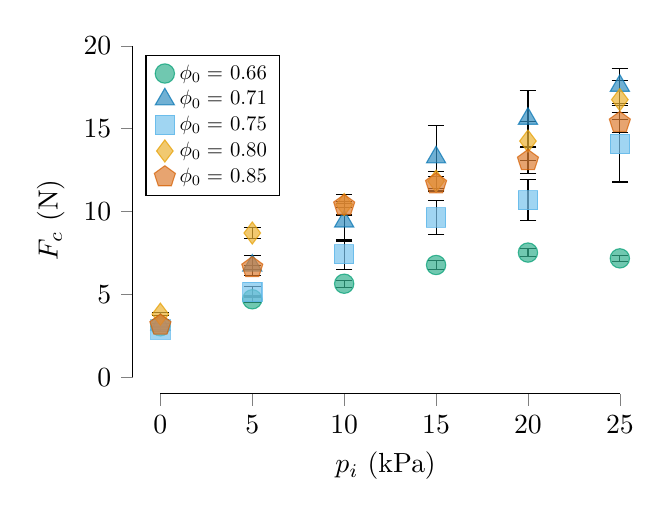
\begin{tikzpicture}
		\begin{axis}[
			%title={Diagonal View - 20 mm section},
			height=6cm,
			width=8cm,
			enlargelimits=false,
			tick pos=left, %
			tick align=outside, %
			axis line style={opacity=0}, %
			after end axis/.code={
				\draw ({rel axis cs:0,0}
				-|{axis cs:0,0}) % xmin (line starts here)
				-- ({rel axis cs:0,0}
				-|{axis cs:25,0}); % xmax (line stops here)
				\draw ({rel axis cs:0,0}
				|-{axis cs:0,0}) % ymin (line starts here)
				-- ({rel axis cs:0,0}
				|-{axis cs:0,20}); % ymax (line stops here)
			},
			legend style={
				at={(0.025,0.975)},
				anchor=north west,
				fill=none
			},
			ylabel={$F_c$ (N)},
			xlabel={$p_i$ (kPa)},
			xmin=-1.5, xmax=26,
			ymin=-1, ymax=20,
			mark size=3pt,
			scatter/classes={
				a={mark=*, mark size=3.5pt, color = Okabe1, fill=Okabe1!80,opacity=0.7},
				b={mark=triangle*, mark size=4pt,color = Okabe2, fill=Okabe2!80,opacity=0.7},
				c={mark=square*, mark size=3.5pt,color = Okabe3, fill=Okabe3!80,opacity=0.7},
				d={mark=diamond*, mark size=4pt,color = Okabe4, fill=Okabe4!80,opacity=0.7},
				e={mark=pentagon*, mark size=4pt,color = Okabe5, fill=Okabe5!80,opacity=0.7},
				f={mark=mystar, mark size = 5pt, color = Okabe6, fill=Okabe6!80,opacity=0.7}
			}
			]
			\addplot[scatter,only marks,% 
			scatter src=explicit symbolic, % Needed for scatter class styling
			error bars/.cd,
			x dir=both, x explicit,
			y dir=both, y explicit
			] 
			table[y error index=2, meta=label] {
				x 	y 		yerr 	label
				%0	2.82	0.40	0.49
				%5	3.45	0.15	0.49
				%10	4.17	0.35	0.49
				%15	4.04	0.08	0.49
				%20	5.31	0.54	0.49
				%25	5.42	0.58	0.49
				
				%0	2.58	0.02	0.58
				%5	3.37	0.16	0.58
				%10	4.13	0.33	0.58
				%15	4.19	0.10	0.58
				%20	4.67	0.22	0.58
				%25	5.46	0.49	0.58
				
				%0	3.07	0.01	0.65
				%5	4.70	0.20	0.65
				%10	5.64	0.21	0.65
				%15	6.77	0.25	0.65
				%20	7.52	0.25	0.65
				%25	7.17	0.20	0.65
				
				0	3.07	0.01	a
				5	4.70	0.20	a
				10	5.64	0.21	a
				15	6.77	0.25	a
				20	7.52	0.25	a
				25	7.17	0.20	a
								
				0	3.18	0.30	b
				5	6.73	0.59	b
				10	9.40	1.18	b
				15	13.27	1.90	b
				20	15.60	1.71	b
				25	17.59	1.05	b
				
				0	2.87	0.12	c
				5	5.14	0.33	c
				10	7.42	0.91	c
				15	9.63	1.01	c
				20	10.68	1.23	c
				25	14.08	2.30	c
				
				0	3.80	0.10	d
				5	8.70	0.32	d
				10	10.42	0.63	d
				15	11.83	0.58	d
				20	14.25	1.16	d
				25	16.75	1.18	d
				
				0	3.14	0.11	e
				5	6.61	0.11	e
				10	10.36	0.12	e
				15	11.66	0.47	e
				20	13.07	0.78	e
				25	15.37	0.62	e
				
				
											
			};
			\addlegendentry[scale=0.75]{$\phi_0=$~0.66}
			\addlegendentry[scale=0.75]{$\phi_0=$~0.71}
			\addlegendentry[scale=0.75]{$\phi_0=$~0.75}
			\addlegendentry[scale=0.75]{$\phi_0=$~0.80}
			\addlegendentry[scale=0.75]{$\phi_0=$~0.85}
		\end{axis}
		
	\end{tikzpicture}
	
	
\end{document}